\documentclass{article}

% if you need to pass options to natbib, use, e.g.:
%     \PassOptionsToPackage{numbers, compress}{natbib}
% before loading neurips_2020

% ready for submission
% \usepackage{neurips_2020}

% to compile a preprint version, e.g., for submission to arXiv, add add the
% [preprint] option:
%     \usepackage[preprint]{neurips_2020}

% to compile a camera-ready version, add the [final] option, e.g.:
%     \usepackage[final]{neurips_2020}

% to avoid loading the natbib package, add option nonatbib:
\usepackage{format}

\usepackage[utf8]{inputenc} % allow utf-8 input
\usepackage[T1]{fontenc}    % use 8-bit T1 fonts
\usepackage{hyperref}       % hyperlinks
\usepackage{url}            % simple URL typesetting
\usepackage{booktabs}       % professional-quality tables
\usepackage{amsfonts}       % blackboard math symbols
\usepackage{nicefrac}       % compact symbols for 1/2, etc.
\usepackage{microtype}      % microtypography
\usepackage{graphicx}
\usepackage{xcolor}
\hypersetup{
	colorlinks,
	linkcolor={red!50!black},
	citecolor={blue!50!black},
	urlcolor={blue!80!black}
}

\title{Generative Vector Art}

% The \author macro works with any number of authors. There are two commands
% used to separate the names and addresses of multiple authors: \And and \AND.
%
% Using \And between authors leaves it to LaTeX to determine where to break the
% lines. Using \AND forces a line break at that point. So, if LaTeX puts 3 of 4
% authors names on the first line, and the last on the second line, try using
% \AND instead of \And before the third author name.

\author{
	Ivan Puhachov \\ 
	UdeM \\
	ivan.puhachov@umontreal.ca \\
}

\begin{document}
	
	\maketitle
	
	\begin{abstract}
		Vector graphics allows for editing without loss of quality. It stores images as a collection of primitives (lines, bezier curves, circles, etc.) with corresponding control parameters (color, width, control points).
		
		Typical generative models are trained on raster images (image as array), while vector graphics space is non-euclidean and thus more challenging. Several approaches were tried, until finally a differentiable rasterizer proposed in \cite{diffsvg} made it possible to do a direct backpropagation to primitives parameters. 

		In this project we apply differentiable rasterizer from \cite{diffsvg} to experiment with generative art on different datasets, GAN architectures, and create adversarial examples using painting. We show that it may become a nice tool in media art creation, as it connects capable GANs and other neural nets with all the advantages of vector graphics.
	\end{abstract}

	\begin{figure}[h]
		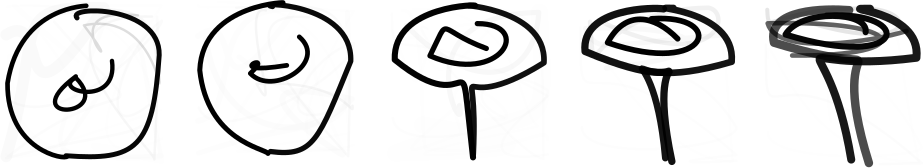
\includegraphics[width=0.45\linewidth]{img/my_plot_vector.png}
		\hspace{4mm}
		\unskip\ \vrule\
		\hspace{4mm}
		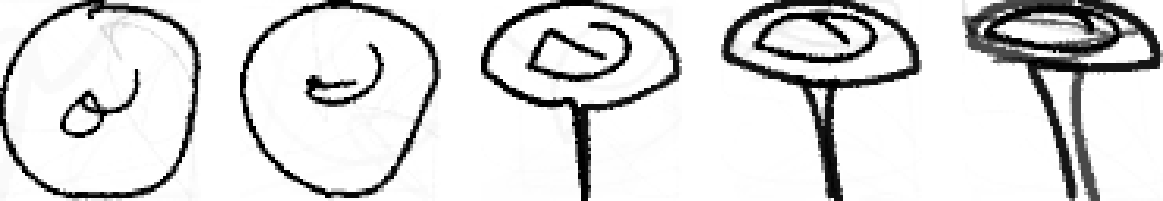
\includegraphics[width=0.45\linewidth]{img/my_plot_raster.png}
		\caption{Interpolation of the latent space in a trained GAN. Typical raster GAN can only generate images of fixed resolution (right), while our Vector GAN model outputs a control parameters for underlying primitives, thus allowing to rasterize image at any resolution (right)}
		\label{fig:inter}
	\end{figure}
	
	\section{Overview}
	Scalable vector graphics (SVG) stores graphics as a collection of drawing primitives (i.e. straight lines, bezier curves, circles) and associated stroke parameters (i.e. color, width, filling color). To view svg grapics we rasterize it - define a canvas of pixels and compute its colors by placing specified primitives. In principle we can rasterize image at any resolution, which is beneficial for art creation and distribution. We can also flawlessly edit vector grapics part by part by modifying its parameters. On the contrary, typical raster graphics (image as array of pixels) has fixed resolution. 
	
	Sketch generation is a known problem, however lack of massive drawing datasets makes it less popular than general image generation. Sketches are hard to process by machine as they use high-level abstractions to convey shapes and depth information, support structures and auxiliary lines. When it comes to sketch generation in vector form, only few works are known, as now data representation is another huge problem. To apply any machine learning on the task of vector image generation, we should have a way to differentiably rasterize vector image. If we have that, generated image can be compared to some ground truth raster image, and error term can be backpropagated down to the underlying vector primitives parameters. Recent advancement  \cite{diffsvg} introduces such a differentiable rasterizer capable of working with different tools and shapes. They show that such rasterizer can be incorporated in the existing generative pipelines. Provided experiments are rather "proof-of-concept" that we wish to explore and expand.
	
	In this work we convey the following experiments:
	
	\begin{itemize}
		\item We train a generative model operating on Bezier curves and circles to show capability of such models.
		\item We train several GAN architectures to generate simple shapes from QuickDraw dataset. We show that such GANs are capable of generating simple sketches of different classes, although with the cost on computations. We compare them using Inception Score and Frechet Inception Distance.
		\item We show how this differentiable rasterizer can be used to generate artistic images
		\item We show that differentiable rasterizer can be used to create adversarial examples in different settings
	\end{itemize}

	Our original project proposal consisted of results replication and changing the dataset to a more complex one. Upon doing the project we realized that it can be expanded to more experiments and novel application. However, experiments with complex dataset are inconclusive due to computational limitations and we discuss it later on.
	
	Overall, we perform several experiments in different setting aiming to achieve meaningful generative art in a vector form, which is a challenging field. We provide visualization of our experiments and the code can be accessed on github repo \href{https://github.com/ivanpuhachov/ift6756}{ivanpuhachov/ift6756}
	
	\subsection{Related works}
	
	Most generative adversarial networks are generating raster images. DoodlerGAN \cite{doodlergan} aimed to replicate human drawings by generating raster body parts. Their generative model DoodlerGAN was trained on a newly collected expressive dataset "Creative Birds" (see samples on Figure \ref{fig:doodlergan}). The generation is then done by 2-stage process: the first net decides what bodypart to redraw, the second net (GAN) generates and updates the corresponding layer. Although results are great, this is hardly different to any other image generation problem, as it neglects the underlying stroke structure and uses raster representation.
	
	\paragraph{SketchRNN} \cite{sketchrnn} modeled drawing as a decision making sequential process and trained seq2seq RNN VAE to generate quick sketches. They train their model on image classes from massive dataset "Quick Draw" of 50,000,000 quick sketches. Drawings are represented as a sequence of $(\Delta x, \Delta y, p_1, p_2, p_3) \in \mathbf{R}^5$ points, where the offset vector $(\Delta x, \Delta y)$ shows the distance from the previous point, and point class vector $(p_1, p_2, p_3)$ shows the current pen state (drawing line, move to the other stroke, finish the drawing). Encoder part is a bidirectional RNN that projects points sequence into representation $h$, which is then linearly projected into $\mu \in \mathbf{R}^{128}$ and $\sigma \in \mathbf{R}^{128}$. We sample a latent representation $z$ from $\mathcal N(\mu, \sigma)$ and pass it to decoder. The decoder goal is to reconstruct the input image with unidirectional RNN, having as input the previous point predicted and the latent representation. SVG VAE \cite{svgvae} applies the same approach to model fonts as a sequence of 4 commands. SketchBERT \cite{sketchbert} moved to a next level by training a giant BERT model on the same QuickDraw data with the same representation. DeepSVG \cite{carlier2020deepsvg} uses transformers to generate SVG control commands for a vider family of svg primitives. Overall, this family of works can be interpreted as a general approach of "get SVG as a sequence of drawing commands, and train a model to replicate it".
	
	\paragraph{Reinforcement learning} was also applied to drawing generation, following the idea that drawing is a sequential decision-making process - see SPIRAL by \cite{ganin2018synthesizing} and SPIRAL++ \cite{mellor2019unsupervised}. These systems are expensive to train, as reinforcement agent receives feedback only in the end of drawing process, thus a lot of training attempts is required. They also follow the approach of drawing as sequence of decision making procedures.
	
	\paragraph{Differentiable rasterizer} proposed in \cite{diffsvg} allows gradient flow from rendered image to svg parameteres, thus we can optimize svg primitives directly from raster signal. Differentiable rasterizer was built by using differentiable iterative solvers (to compute the distance to analytical primitive) and computing pixel color as an integral over its area. Details of their implementation is beyond the scope of this project, and we refer to the original paper and their open repository \url{https://github.com/BachiLi/diffvg} to use differentiable rasterization module. What is important is that this rasterizer supports wide range of primitives. GAN results were proposed, see reported  results on Figure \ref{fig:diffsvg}
	
	Finally, very recent Im2Vec \cite{reddy2021im2vec} uses differentiable rasterizer from \cite{diffsvg} to generate vector graphics from raster examples.
	
	\begin{figure}[h]
		\centering
		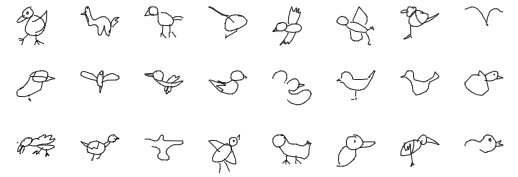
\includegraphics[width=0.55\textwidth]{img/quickdraw.png}
		\hspace{4mm}
		\unskip\ \vrule\
		\hspace{4mm}
		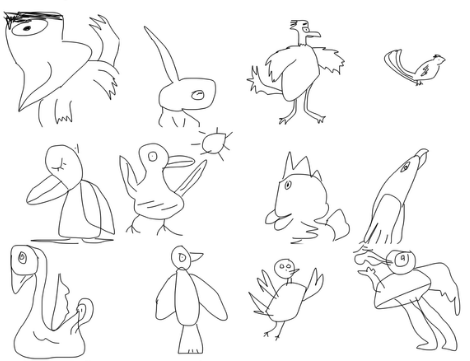
\includegraphics[width=0.25\textwidth]{img/data_birds.png}
		\caption{On the left: quickdraw dataset samples of category "bird" , on the left - samples from Creative Birds dataset by \cite{doodlergan}}
		\label{fig:doodlergan}
	\end{figure}

\section{GAN Experiments}
	\paragraph{Dataset}
	We took simple sketches from QuickDraw dataset with categories "apple", "cookie", "donut", "face", "lollipop" and 5000 of each category with resolution 64x64. See examples on Figure \ref{fig:dataset}. Note that we train a "grayscale" model to save computations and fit to grayscale dataset, while it is possible to have colored sketches.
	
	We also tried training on more complex classes like "owl" or another dataset Creative Birds, but due to computational limitations our model did not converge to any good looking results. Learning dynamics and our experience with simpler dataset suggest that we simply need to train it for longer time. See examples of undertrained model on Figure \ref{fig:gen_creative}.
	
	 \begin{figure}[h]
	 	\centering
	 	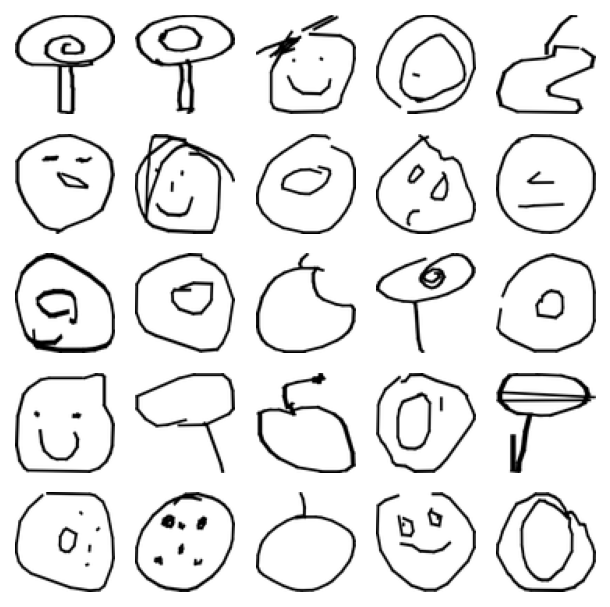
\includegraphics[width=0.45\textwidth]{img/data.png}
	 	\hspace{4mm}
	 	\unskip\ \vrule\
	 	\hspace{4mm}
	 	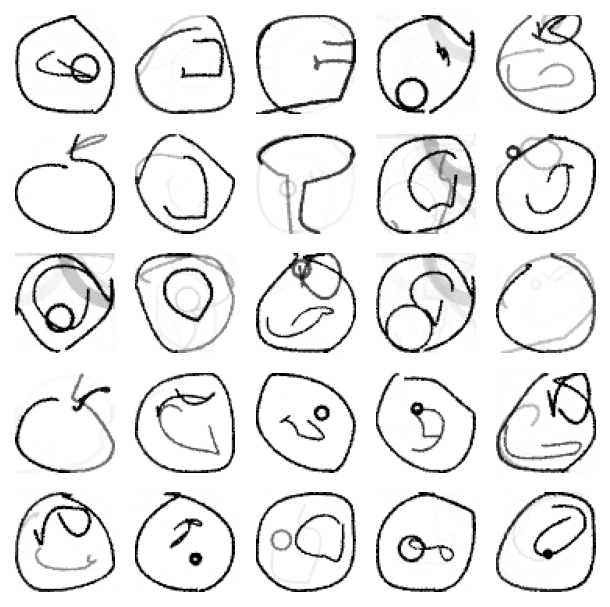
\includegraphics[width=0.45\textwidth]{img/gen.png}
	 	\caption{On the left - samples of our dataset: "apple", "cookie", "donut", "face", "lollipop" categories of QuickDraw dataset. On the right -- generated examples}
	 	\label{fig:dataset}
	 \end{figure}
	
	\paragraph{Architectures}
	Generator takes as input a latent vector $z \in \mathbf{R}^100$ and outputs parameters for 16 bezier curves (14 positional parameters + width and alpha) and 5 circles (2 positional parameters + radius + width + alpha).   Neural net consists of 4 flat linear layers of dimensions [128, 256, 512, 1024], the last layer is then projected into each parameter family independently. Output parameters is then grouped and passed to differentiable rasterizer to generate image.
	
	Discriminator is a convolutional neural network of 6 layers, with LeakyReLU activation. After experiments we ended up using the same discriminator architecture as was proposed in the original paper, as our attempts failed due to discriminator net being too powerful.
	
	We implemented and trained the following modifications for training GAN, commonly used in literature.
	
	Training of each model took approximately 10 hours on a single GPU (NVidia RTX2080Ti). Unfortunately, we could not use Google Colab as differentiable rasterizer was not compatible with Colab hardware. 
	
	\paragraph{WGAN} \cite{arjovsky2017wasserstein} makes a critic $K$-Lipschitz by clipping its gradients to stabilize training 
	$$\omega \leftarrow clip (\omega, -0.01, 0.01)$$
	
	\paragraph {WGAN-GP} \cite{gulrajani2017improved} forces $K$-Lipschitz by adding a gradient penalty to the loss
	$$\hat x \leftarrow \epsilon x_{real} + (1-\epsilon) x_{fake}$$ 
	$$loss \leftarrow D(x_{fake}) - D(x_{real}) + \lambda (\| \nabla_{\hat x} D(\hat x) \|_2 - 1)^2$$
	
	\paragraph {SNGAN} \cite{miyato2018spectral} Force 1-Lipschitz continuity by spectral normalization of critic's layers
	$$\bar W_{SN} (W) = \frac W {\sigma(W)} $$
	
	\paragraph {LOGAN} \cite{wu2020logan} More gradient flow to generator by making a latent gradient step $z = z + \Delta z$ before passing image to discriminator
	$$g = \frac{\partial D(G(z))}{\partial z}; \; \; \Delta z = \frac {\alpha} {\beta + \| g \|^2} \cdot g$$
	
	\paragraph{Evaluation}
	We evaluated and compared our models using Inception Score and Frechet Inception distance. Inception Score uses pretrained classificator and measures the variety of generated examples through measuring distribution of labels predicted by pretrained classifier. Frechet inception distance measures this variety by comparing feature distribution extracted by classifier on validation set and generated samples:
	$$\| \mu_{real} - \mu_{fake} \|_2^2 + Trace(\Sigma_{real} + \Sigma_{fake} - 2 (\Sigma_1 \Sigma_2)^{0.5})$$
	
	FID score between validation and test subsets is 30.56
	
	\paragraph{Results}
		\begin{table}[]
		\centering
		\begin{tabular}{lll}
			\textbf{Model} & \textbf{IS} & \textbf{FID} \\
			WGAN           & 1.935       & 94.14        \\
			WGAN-GP        & 1.856       & 101.7        \\
			SN WGAN-GP     & 1.919       & 84.54        \\
			LOGAN NGD      & 1.11        & 208         
		\end{tabular}
		\caption{Qualitative results of training on a fixed dataset with the same hyperparameters}
		\label{tab:res}
	\end{table}
	Qualitative results are reported in Table \ref{tab:res}. 
	
	We see that LOGAN is much worse in scores, and indeed the model failed to converge to meaningful results, generating the same repeating pattern. This is known as mode collapse problem. We see no theoretical limitations with using this approach, some hyperparameter tweaking is required to make it work, as we spent a lot of time finding the correct batch size and learning rate to make other models work.
	
	As for Wasserstein GANs, they showed good convergence and results, but results are far from perfect both visually and qualitatively. We did not achieve desired FID score of 30 (as between validation and test subsets). But again, we assume that it is only the matter of longer training.
	
	\paragraph{Latent space exploration} As generator's output now has a direct meaning (it is connected to control parameters of underlying primitives), opposed to raster GAN's, which generate pixel colors directly, we see extracting meaningful directions in a latent space as promising direction of future research. See example of latent space interpolation on figure \ref{fig:inter}.
	
	\paragraph{Conclusions} Differentiable rasterization is computationally expensive operation and thus GAN with vector graphics takes approximately 10 times more time to converge. Unfortunately, we could not speed up this process as increasing batch size breaks the training dynamics. More research is required in this part.
	

\section{Adversarial examples}
Adversarial examples are well known problem in machine learning. In essence, we take a picture and slightly change pixel colors such that some targeted model fails to classify object correctly. Methods like Fast Gradient Sign were proposed in \cite{goodfellow2015explaining} and many more were developed afterwards. In the simples scenario, we have complete access to classification model. Fast Gradient Sign method proposes changing the image in the direction of gradient of model's loss with respect to the input image $x$.
$$x_{new} = x + \epsilon sign(\nabla_x J (\theta, x, y))$$
Where $y$ is the correct label of the image $x$. 

We first tried to replicate impressive results of FGSM but with vector curves. To do this we fit curves to some predefined image. This was also done in the reference paper and is named "painterly rendering". See Figure \ref{fig:paint}. We start with randomly initialized Bezier curves and fit their parameters to match with some target image, with loss computed as $L_2$ difference between target image and the rasterized one.

Having vector image resembling the targeted one, we can fix some parameters (i.e. colors and line widths) and simply change the remaining ones (control points) in the direction of targeted image class. We do this by making gradient steps toward maximizing the probability our pre-trained model (InceptionV3) assigns to desired class. See figure \ref{fig:advex}.

Another experiment we did with adversarial examples was to limit the starting amount of curves and try to generate adversarial examples from scratch. We find that this approach does not converge to any class. Instead, if we take few steps of painterly rendering towards some fixed image, and then guide parameters update with classification model gradient we can achieve some abstract images, like the rightmost image on figure \ref{fig:advex}. We assume this may be an example of good initial guess rather and willing to explore it in our future work.

\begin{figure}
	\centering
	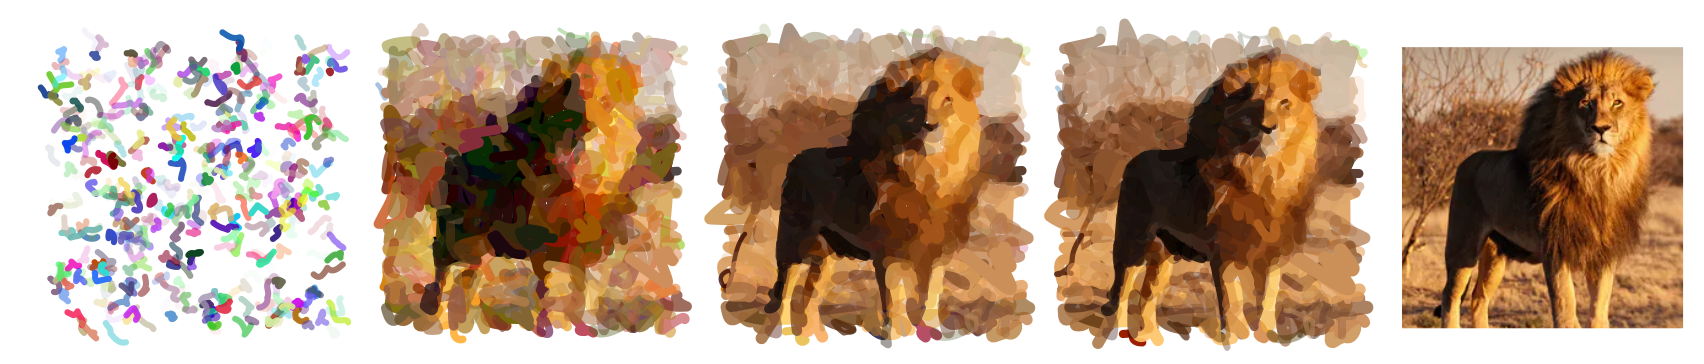
\includegraphics[width=0.9\linewidth]{img/paint_iterations.png}
	\caption{Painterly rendering example: starting from randomly initialized bezier curves we optimize for svg parameters (contol points, color, width) such that generated image is matching the target one (leftmost) as $L_2$ distance between matrics. From left to right: initialization, 50 optimization steps, 100 steps, 200 steps, target image}
	\label{fig:paint}
\end{figure}

\begin{figure}
	\centering
	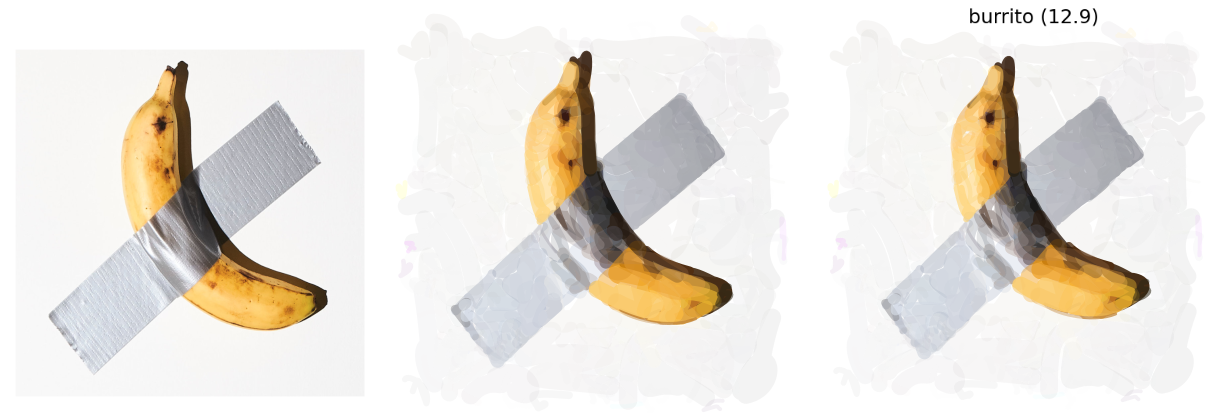
\includegraphics[width=0.7\linewidth]{img/adversarial.png}
	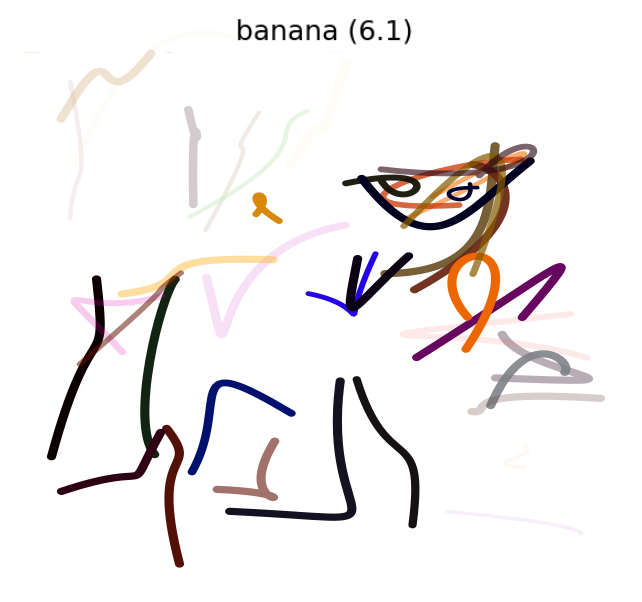
\includegraphics[width=0.25\linewidth]{img/banana.png}
	\caption{Examples of adversarial attacks. Leftmost: target image, that we approximate with painterly rendering. We then optimize for control points (fixing colors and widths) such that the resulting image is classified as "burrito". If we limit the number of strokes, do only a few painterly steps towards some image (in this case, lion) and then rely only on classification model gradients, we achieve some highly abstract drawing that is still classified as a banana (rightmost)}
	\label{fig:advex}
\end{figure}

Our last experiment, that we call "Adversarial Vandal" consists of drawing only a few strokes on top of some image to force classification model to make mistakes. See results on Figure \ref{fig:advvan}.

\begin{figure}
	\centering
	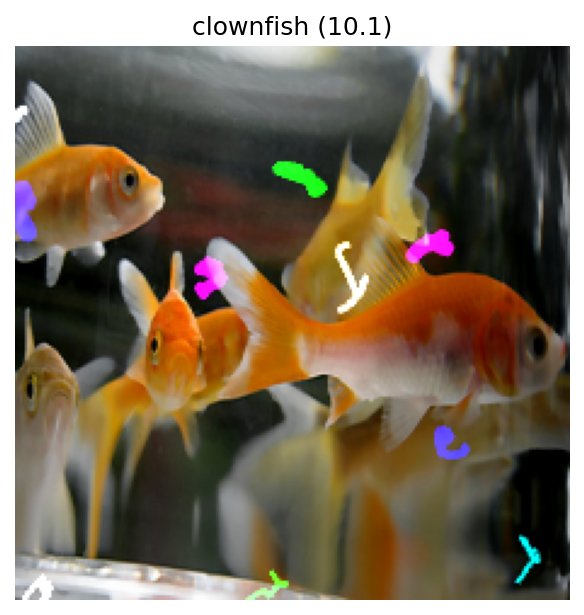
\includegraphics[width=0.3\linewidth]{img/vandal.png}
	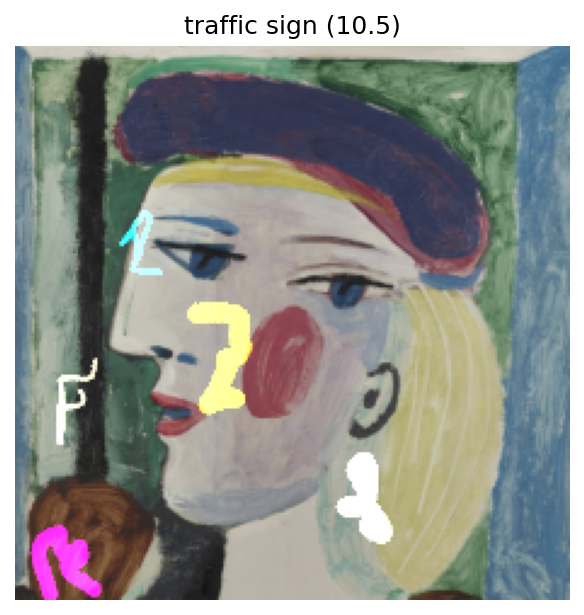
\includegraphics[width=0.3\linewidth]{img/vandal1.png}
	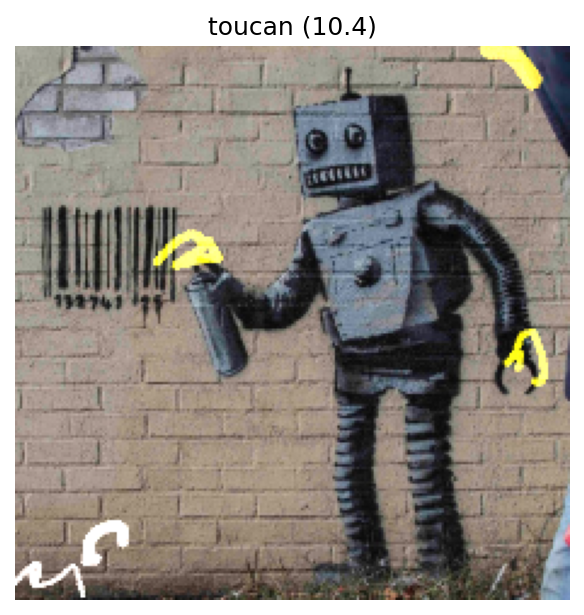
\includegraphics[width=0.3\linewidth]{img/vandal2.png}
	\caption{Adversarial vandal examples. 10 bezier curves are drawn on top of an image such that classification model InceptionV3 is fooled towards specified class}
	\label{fig:advvan}
\end{figure}

\section{Future work}
\paragraph{Latent space directions} As we have direct connection between generator output and rasterized images, we expect that resulting latent space has meaningful directions. We may employ some specialized training techniques, like recently published \cite{he2021eigengan} to force meaningful directions. Resulting model can be applied for animation purposes.

\paragraph{Meaningful adversarial examples} Inspired by artwork on Figure \ref{fig:face}, we will continue the experiments with adversarial examples aiming to automatically generate some human-readable vector art.


\section{Conclusion}

\paragraph{Code} Code is available in this github repository: \url{https://github.com/ivanpuhachov/ift6756}. We used differentiable rasterizer provided in \cite{diffsvg} and consulted with their model architectures on github \url{https://github.com/BachiLi/diffvg}, the rest of the code is our own, proper credits are mentioned.

We trained and evaluated several GAN models in a field of vector image generation. Despite being trained with 64x64 px image dataset, such model can generate sketches at any resolution, due to using vector graphics. Models showed good generalization ability, generating images of different classes, but more training is required to perfect the results. 

We show that differentiable rasterizer can be applied for generating adversarial examples and we will proceed in this direction to generate good-looking vector images.


	
	\bibliography{example_paper}
	\bibliographystyle{abbrvnat}
	
	\begin{figure}[h]
		\centering
		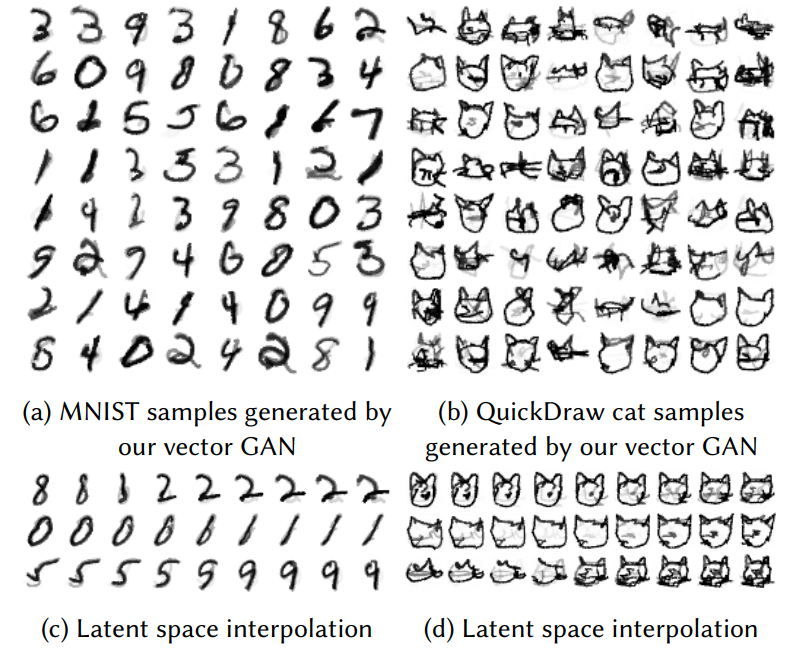
\includegraphics[width=0.65\textwidth]{img/diffsvg.png}
		\caption{Samples generated by GANs, screenshot directly from a paper by \cite{diffsvg}}
		\label{fig:diffsvg}
	\end{figure}
	
	\appendix 
	
	
	\begin{figure}[h]
		\centering
		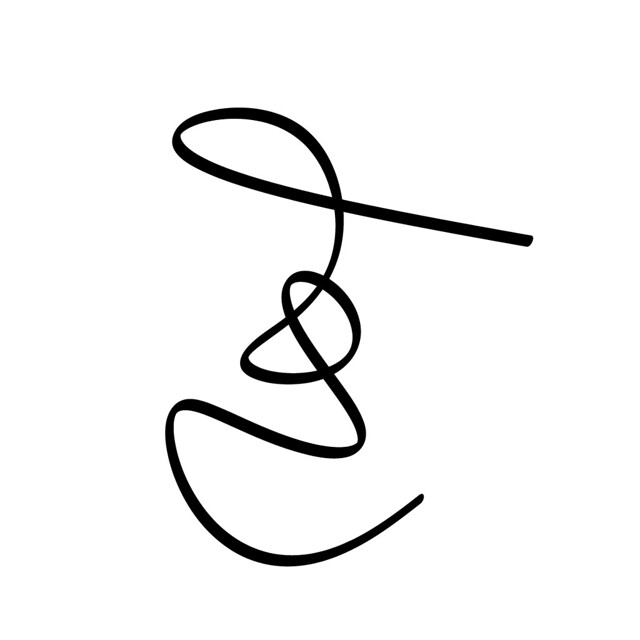
\includegraphics[width=0.55\textwidth]{img/face.jpg}
		\caption{"Evolutionary Faces (2020). A curve generator is pitted against a face recognition algorithm. Using an evolutionary process, the curves thrive to be more face-like. Limiting the curve to just a single or double line forces the generator to remain abstract". Description and image are taken from \href{http://www.aiartonline.com/highlights-2020/matty-mariansky/}{NeurIPS20 workshop}, art by Matty Mariansky}
		\label{fig:face}
	\end{figure}

\begin{figure}[h]
	\centering
	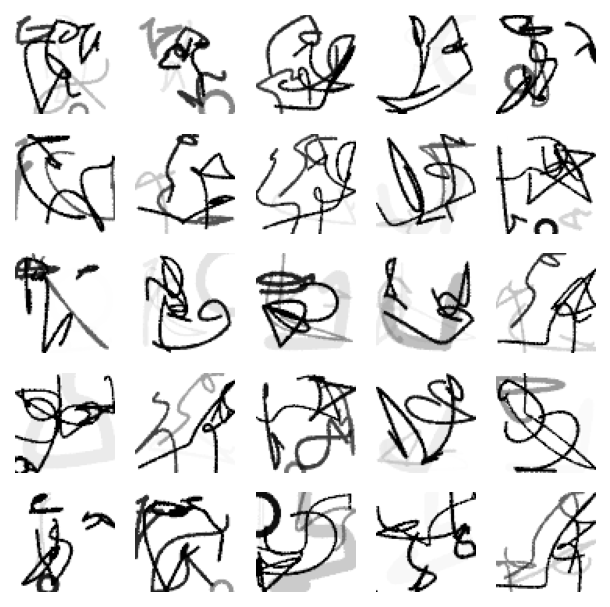
\includegraphics[width=0.45\textwidth]{img/gen_cr.png}
	\caption{Generated samples of model trained on Creative Birds dataset.}
	\label{fig:gen_creative}
\end{figure}
	
\end{document}